% based on a template made by the university of cologne
% http://www.mi.uni-koeln.de/wp-MIEDV/wp-content/uploads/2016/07/LaTeX-Vorlage.zip - 2023-11-02
\documentclass[12pt,a4paper]{scrartcl}

\addtokomafont{sectioning}{\rmfamily}
\usepackage[ngerman]{babel}% deutsches Sprachpaket wird geladen
\usepackage[T1]{fontenc} % westeuropäische Codierung wird verlangt
\usepackage[utf8]{inputenc}% Umlaute werden erlaubt
\usepackage[usenames]{color} % Erlaubt die Benutzung der namen im Farbpaket und deren Änderung
\usepackage{amsmath} % Erweiterung für den Mathe-Satz
\usepackage{amssymb} % alle Zeichen aus msam und msmb werden dargestellt
\usepackage{graphicx} % Graphiken und Bilder können eingebunden werden
%\usepackage{multirow} % erlaubt in einer Spalte einer Tabelle die Felder in mehreren Zeilen zusammenzufassen
\usepackage{enumerate} % erlaubt Nummerierungen
\usepackage{xurl} % Dient zur Auszeichnung von URLs; setzt die Adresse in Schreibmaschinenschrift.
\usepackage[center]{caption}  % Bildunterschrift wird zentriert
%\usepackage{subfigure} % mehrere Bilder können in einer fugure-Umgebung verwendet werden
%\usepackage{longtable} % Diese Umgebung ist ähnlich definiert wie die tabular-Umgebung, erlaubt jedoch mehrseitige Tabellen.
%\usepackage{paralist} % Modifikation der bereits bestehenden Listenumgebungen
\usepackage{lmodern}% Für die Schrift
\usepackage[hidelinks]{hyperref} % Links und Verweise werden innerhalb von PDF Dokumenten erzeugt
%\usepackage{wrapfig} % Das Paket ermöglicht es von Schrift umflossene Bilder und Tabellen einzufügen.
\usepackage{latexsym} % LaTeX-Symbole werden geladen
\usepackage{tikz} % Erlaubt es mit tikz zu zeichnen
\usepackage{tabularx} % Erlaubt Tabellen
\usepackage{algorithm} % Erlaubt Pseudocode
\usepackage{color} % Farbpaket wird geladen
%\usepackage{stmaryrd} % St Mary Road Symbole werden geladen
\usepackage{physics}
\usepackage[version=4]{mhchem} % Chemie: \ce & \pu

\numberwithin{equation}{section} % Nummerierungen der Gleichungen, die durch equation erstellt werden, sind gebunden an die section
\newcommand{\HRule}{\rule{\linewidth}{0.7mm}}

\hypersetup{
  pdftitle={B1.5: Elektronenspinresonanz},
  pdfcreator={\LaTeX}
}

\setcounter{secnumdepth}{6}
\setcounter{tocdepth}{6}

\begin{document}
\begin{titlepage}
	\pagestyle{empty}

	\begin{center}

	\textsc{\LARGE Universität zu Köln }\\ [0.4cm]
	\textsc{Mathematisch--Naturwissenschaftliche Fakultät} \\[1.5cm]

	
\includegraphics[width=0.45\textwidth]{../media/uni.jpg} \\[1.5cm]  % Uni-Logo wird geladen

	\textsc{\Large Praktikum~B}\\[2mm]
	\textsc{28. Mai 2024}\\[10mm]
	\HRule \\[0.4cm]

		{	\Huge \bfseries B1.5}\\[0.4cm]
			{	\huge \bfseries Elektronenspinresonanz}\\[0.3cm]
	
	\HRule \\[3cm]

 	\begin{center}
		\textsc{\Large Catherine~Tran } \\[3pt]
		\textsc{\Large Carlo~Kleefisch } \\[3pt]
		\textsc{\Large Oliver~Filla } \\[3pt]
	\end{center}
	\end{center}
\end{titlepage}

\newpage
\tableofcontents
\newpage

\clearpage
\hypertarget{einleitung}{%
\section{Einleitung}\label{einleitung}}

Die Elektronenspinresonanz (ESR) ist eine Hochfrequenzspektroskopiemethode, welche das Untersuchen von Eigenschaften paramagnetischer Proben ermöglicht. Sie basiert auf dem Zeeman--Effekt, der die Aufspaltung von Energieniveaus in einem äußeren Magnetfeld begründet.

Bei der ESR kann man Übergänge zwischen Zeeman--Niveaus mit gleicher Hauptquantenzahl beobachten, indem die resonante Absorption von Mikrowellen beobachtet wird.

Durch das aufgezeichnete Absorptionsspektrum lässt sich weiterhin der Landé--Faktor bestimmen.

\clearpage
\hypertarget{theoretische-grundlagen}{\section{Theoretische Grundlagen}\label{theoretische-grundlagen}}

\hypertarget{elektromagnetismus}{\subsection{Elektromagnetismus}\label{elektromagnetismus}}

\hypertarget{dipolmoment}{\subsubsection{Dipolmoment}\label{dipolmoment}}

Das magnetische \emph{Dipolmoment} $\vec \mu$ tritt auf, wenn sich elektrische Ladungen bewegen. Es lässt sich über das auf einen magnetischen Dipol wirkende Drehmoment $\vec \tau$ in einem Magnetfeld $\vec B$ definieren.

Für eine ebene Leiterschleife ist es folgendermaßen beschrieben. \cite{Jackson} Damit ist das Dipolmoment $\vec \mu$ parallel zum Drehimpuls $\vec{L}$. Die Energie $E$ zur Ausrichtung eines Dipolmomentes wird durch das Skalarprodukt $\vec \mu \cdot \vec B$ beschrieben.

\begin{eqnarray}
	\vec \tau &=& \vec \mu \times \vec B \\
	E &=& \vec \mu \cdot \vec B \label{eq:EDipol}
\end{eqnarray}

\noindent
Das magnetische Moment eines Atoms wird durch Rotation einer elektrischen Ladung erzeugt. Beispielsweise entsteht im Bohr--Sommerfeld'schen Atommodell das \emph{Bohr'sche Magneton} $\mu_B$ durch die Rotation eines Elektrons um den Atomkern. Es wird durch die reduzierte Planck--Konstante $\hbar$, die Elementarladung $e$ und die Elektronenmasse $m_e$ beschrieben.

\begin{eqnarray}
	\mu_B &=& \frac{e\hbar}{2m_e}
\end{eqnarray}

\hypertarget{spin}{ \subsubsection{Spin}\label{spin}}

Der Spin $\vec s$ ist der Drehimpuls, der durch die Rotation eines Körpers um sich selbst entsteht. Er kann nur einen von zwei Werten abnehmen.

Beispielsweise beträgt der Eigenwert des Elektronenspins immer $\pm\frac{\hbar}{2}$, insbesondere gilt für die $z$--Komponente des Spins $\hat s_3\ket{z\pm}=\pm\frac{\hbar}{2}\ket{z\pm}$. Dadurch ist die magnetische Quantenzahl $m=\pm\frac{1}{2}$. Da $j$ die Grenzen der gültigen $m$ definiert, muss die Drehimpulsquantenzahl $j=s=\frac{1}{2}$ sein. Dies wird als Spin bezeichnet.

Elektronen nennt man \emph{Spin-$\frac{1}{2}$--Teilchen} oder Fermionen, da der Spin $s=\pm\frac{1}{2}$ halbzahlig ist.

Das Dipolmoment $\vec \mu$ und der Spin $\vec s$ sind über das \emph{gyromagnetische Verhältnis} $\gamma$ miteinander verknüpft. Dazu wird der \emph{Landé--Faktor} $g$ benötigt.

\begin{eqnarray}
	\vec \mu &=& \gamma \vec{s} \label{eq:dipolmomentSpin} \\
	\gamma &=& \frac{g\mu_B}{\hbar} \label{eq:gyromag} \\
	g &=& 1 + \frac{j(j+1) + s(s+1) + l(l+1)}{2j(l+1)}
\end{eqnarray}

\noindent
Hierbei werden die Eigenwerte der Drehimpulsoperatoren $\hat{\vec j},\hat{\vec s},\hat{\vec l}$ benötigt, die den Spin $\vec s$, den Bahndrehimpuls $\vec l$ und den Gesamtdrehimpuls $\vec j = \vec l + \vec s$ beschreiben. Falls es keinen Bahndrehimpuls $l=0$ gibt, so folgt $g=2$.

\hypertarget{zeemanneffekt}{\subsubsection{Zeemann--Effekt}\label{zeemanneffekt}}

Nach dem Bohr--Sommerfeldschen Atommodell haben Elektronen durch die Rotation um den Atomkern einen gequantelten Drehimpuls $\vec{L}$. Er ist durch die Quantenzahl $l=1,2,3,\dots$ quantisiert, es gilt $|\vec{L}| = l\hbar$. Die Drehimpulskomponente in Richtung der $z$--Achse $L_z=m\hbar$ ist nun durch eine magnetische Quantenzahl $m=-l,-l+1,\dots,l$ zu beschreiben.

Durch $L_z$ werden die Energieniveaus der Elektronen verschoben. Die Energieverschiebung $\Delta E$ entspricht der Energie, ein Dipolmoment $\vec \mu$ in einem Magnetfeld $\vec B$ auszurichten $\eqref{eq:EDipol}$. Diese Verschiebung führt zu einer Verschiebung der Spektrallinien. Außerdem ist dadurch auch das magnetische Moment gequantelt.

Aufgrund des Zeemann--Effekts kommt es zur Lamorpräzession der Elektronen.

\hypertarget{lamorpruxe4zession}{%
	\subsubsection{Lamorpräzession}\label{lamorpruxe4zession}}

Das magnetische Moment $\mu$ eines Spins im Magnetfeld $\vec{B}$ weist durch Quantenschwebung eine Präzession mit einer \emph{Lamorfrequenz} $\omega_L$ auf. Dies bedeutet, dass der Spin rotiert.

\begin{eqnarray}
	\omega_L &=& \gamma\cdot B
\end{eqnarray}

\subsubsection{Paramagnetismus}
\label{Paramagnetismus}

In einem paramagnetischen Material existieren innere magnetische Dipolmomente, die beispielsweise durch den Spin und den Bahndrehimpuls der Elektronen hervorgerufen werden. Im Gegensatz zum Ferromagnetismus bilden diese jedoch keine kohärenten Domänen, sondern sind zufällig angeordnet. Ein Atom benötigt ungepaarte Elektronen, um ein permanentes Dipolmoment aufzuweisen.

Erst in Anwesenheit eines äußeren Magnetfeldes richten sich die Dipolmomente entlang des Feldes aus. Daher ist die magnetische Suszeptibilität $\chi$ eines Paramagneten positiv. Die Magnetisierung $M$ ergibt sich aus dem Produkt der Suszeptibilität $\chi$ und der magnetischen Feldstärke $H$.

Die Suszeptibilität ist sowohl material- als auch temperaturabhängig. Mit steigender Temperatur erhöht sich die Wahrscheinlichkeit einer antiparallelen Ausrichtung der magnetischen Dipolmomente zum Magnetfeld. Zudem führt die erhöhte thermische Energie zu einer Zunahme der Eigenbewegung der Teilchen, was der Ausrichtung entgegenwirkt. Dadurch nimmt die Magnetisierung ab. Dieses Verhalten wird durch das Curie--Gesetz beschrieben, welches die Curie--Konstante $C$ einführt.

\begin{eqnarray}
	\chi &=& \frac{C}{T}
\end{eqnarray}

\subsubsection{Erdmagnetfeld}
\label{Erdmagnetfeld}
Unsere Erde verhält sich wie ein großer Stabmagnet mit einem starken Magnetfeld.

$95\,\%$ des Feldes entsteht aus Induktionsvorgänge im flüssigen, elektrisch leitfähigen Erdkern. Dieser Prozess wird Geodynamo-Prozess genannt. Magnetisierte Gesteine sowie Felder von Stromsystemen in der Ionosphäre und Magnetosphäre tragen die restlichen $5\,\%$ zum Magnetfeld bei.

Die Stärke des Feldes ist abhängig vom Ort und schwankt stark. Geodynamo--Prozesse polen das Erdmagnetfeld um, was tausende Jahre dauert. Momentan befindet sich der magnetische Nordpol in der Nähe des geografischen Südpols und umgekehrt. Die magnetische Flussdichte beträgt am Äquator etwa $25\,\mu T$ und an den Polen etwa $70\,\mu T$. \cite{Geomagnetismus}

\subsection{Energieniveaus}
\label{Energieniveaus}

\textsc{Max Planck} formulierte um 1900 die Quantenhypothese. Nach dieser können nicht alle physikalischen Größen kontinuierliche Werte nehmen. Das kleinste übertragbare Energiepaket wird durch das Planck'sche Wirkungsquantum $h$ und die Frequenz $\nu$ beschrieben. Daher ist auch die Energie in Atomen gequantelt.

\begin{eqnarray}
	E &=& h\cdot \nu \label{eq:Energie Strahlung}
\end{eqnarray}

\subsubsection{Hauptstruktur}
\label{Wasserstoffatom}
Zur Vereinfachung wird im Folgenden das Wasserstoffatom betrachtet. Dessen Energieeigenwerte sind allein durch die Hauptquantenzahl $n$ bestimmt. Sie wird zudem durch die Rydberg--Konstante $\mathrm{Ry}$ und die Kernladungszahl $Z$ beschrieben.

\begin{eqnarray}
	E_n &=& - \mathrm{Ry} \cdot \frac{Z^2}{n^2} \\
	%&=& -\frac{\hbar^2}{2 \mu a^2 n^2} \\
	\mathrm{Ry} &=& 13.6057 \mathrm{\,eV}
\end{eqnarray}

\noindent
Die Energiedifferenz $E_{21}$ zwischen zwei Energiezuständen entspricht der Energie $\hbar\omega$ des Photons, das bei dem Übergang zwischen den Zuständen erzeugt oder vernichtet wird.

\begin{eqnarray}
	E_{21} &=& \mathrm{Ry} \left( \frac{1}{n_1^2} - \frac{1}{n_2^2} \right)
\end{eqnarray}

\noindent
Die Drehimpulsquantenzahl $l$ erfüllt die Bedingung $l \leq n - 1$, woraus folgende Bedingung für den Entartungsgrad $k$ folgt.

\begin{eqnarray}
	k &=& \sum_{l=0}^{n-1} (2l+1) \\
	k &=& n^2
\end{eqnarray}

\subsubsection{Feinstruktur}
Durch spektrale Hochauflösungsvermögen können kleinere Aufspaltungen in Atomen entdeckt werden. Diese Energien sind viel kleiner als die Energie zwischen zwei benachbarten Schalen. Hauptursache für diese Aufspaltung sind relativistische Korrekturen, die Spin--Bahn--Kopplung sowie weitere Effekte. \cite{Weber}

Den kleinsten Betrag zur Feinstruktur trägt der \emph{spinmagnetische Effekt} bei. Hierbei wechselwirken die Spins ungepaarter Elektronen mit dem von ihnen erzeugten Magnetfeld, dafür erforderlich sind ein Spin $S>0$ und ein Bahndrehimpuls $L\geq 0$. Dieser Effekt lässt sich in diesem Versuch untersuchen, obwohl er sehr klein ist.

Der zweitgrößte Effekt ist die \emph{Spin--Spin--Kopplung}, welche im Wesentlichen die Kopplung vom Spin zweier Elektronen mit der selben Hauptquantenzahl beschreibt. Hierfür müssen für den Spin $S\geq 1$ und $L\geq 0$ für den Bahndrehimpuls gelten. Da in diesem Versuch Radikale untersucht werden, muss dieser Effekt nicht genauer betrachtet werden.

Den größten Effekt bildet die \emph{Spin--Bahn--Kopplung}, bei der der Spin $S>0$ sich mit dem Bahndrehimpuls $L>0$ zu einem Gesamtdrehimpuls $J$ koppelt. Diese Aufspaltung ist so groß, dass sie mit dem ESR nicht untersucht werden kann.

\subsubsection{Hyperfeinstruktur}
Die \emph{Hyperfeinstruktur} entsteht durch Wechselwirkungen des Gesamtdrehimpulses $J$ mit dem Kernspin $I$.

\subsubsection{Auswahlregeln}
Die Auswahlregeln für Energieübergänge bestimmen, ob ein Übergang von einem Zustand in einen anderen stattfinden darf. Damit wird auch die Übergangswahrscheinlichkeit beschrieben.

Für diesen Versuch spielen magnetische Dipolübergänge die zentrale Rolle. Die Auswahlregel lautet hierbei $\Delta m_j = \pm 1$.

\subsubsection{Besetzungszahlen und Boltzmannfaktor}
Die Besetzungszahl gibt die Anzahl $N_i$ der Teilchen in einem Energiezustand $E_i$ im thermischen Gleichgewicht an. Sie wird mithilfe des Boltzmann--Faktors beschrieben, der $E_i$ in Relation zur thermischen Energie $k_bT$ setzt.

\begin{eqnarray}
	N_i &=& \exp(-\frac{E_i}{k_BT})
\end{eqnarray}

\noindent
Das Besetzungsverhältnis zweier Zustände durch ihre Energiedifferenz $\Delta E$ bestimmt. % was ist g_j?

\begin{eqnarray}
	\frac{N_2}{N_1} &=& \exp(-\frac{\Delta E}{k_BT}) \\
		&=& \exp(-\frac{g_j\mu _B B}{k_BT})
\end{eqnarray}

\hypertarget{resonanz}{\subsubsection{Resonanz}\label{resonanz}}

Ganz allgemein ist Resonanz das verstärkte Mitschwingen eines schwingungsfähigen Systems, wenn es einer zeitlich veränderlichen Einwirkung unterliegt. Dabei kann das System um ein Vielfaches stärker ausschlagen als beim konstanten Einwirken der Anregung mit ihrer maximalen Stärke.

Im Falle von ESR werden die magnetischen Dipole von Elektronen resonant angeregt. Dazu sind ungepaarte Elektronen notwendig, die durch Radikale bereitgestellt werden.

Als \emph{Radikale} bezeichnet man Atome oder Moleküle mit mindestens einem ungepaarten Elektron, die meist besonders reaktionsfreudig sind. Radikale werden mit einem Punkt dargestellt, z.B. Stickstoffmonoxid $(\ce{NO^\bullet})$, der das freie Elektron symbolisiert. \cite{Radikale}

\subsubsection{Relaxation und Sättigung}
Relaxation bezeichnet die Abregung eines angeregten Systems durch Photonenabstrahlung, beispielsweise eines Atoms oder Moleküls. Dadurch gelang es in seinen Grundzustand.

Die Zeit zwischen Anregung und Relaxation wird \emph{Relaxationszeit} genannt. Je unwahrscheinlicher ein Übergang ist, desto höher ist die Relaxationszeit. In diesem Versuch sind die magnetischen Übergänge unwahrscheinlich und haben daher eine hohe Relaxationszeit.

Ist die Relaxationszeit hoch, kommt es zu Sättigung. Dabei verschwindet die Besetzungszahldifferenz zwischen Grundzustand und angeregtem Zustand durch ständige Anregungen. \cite{Oldenburg} In diesem Fall wird das ESR--Signal immer kleiner und breiter bis, es irgendwann komplett verschwindet.

\subsection{Linienverbreiterung}
Das ESR--Signal ist nicht beliebig scharf, sondern besitzt eine bestimmte Breite. Nach Heisenberg muss die Energie eine Unschärfe aufweisen, da die Relaxationszeit endlich ist. Die Breite der Resonanzkurve $\Delta \nu $ lässt sich mit der transversalen Relaxationszeit $T_2$ bestimmen, die auch Spin--Spin--Relaxationszeit genannt wird.

\begin{eqnarray}
	\Delta \nu &=& \frac{1}{2 \pi T_2}
\end{eqnarray}

\noindent
Im Unterschied dazu gibt es die Spin--Gitter--Relaxationszeit $T_1$, welche den Grad der Sättigung bestimmt. $T_2$ dagegen führt nicht zur Sättigung.

Diese zwei Prozesse führen zu einer homogenen Linienverbreiterung, die durch eine Lorentz--Kurve angenähert werden kann. Bei Resonanz ohne Sättigung wird die Kurve folgendermaßen beschrieben. \cite{Bern}

\begin{eqnarray}
	f(\omega) &=& \frac{T_2}{\pi}\frac{1}{(1+T_2^{\,2} (\omega - \omega _0)^2)}
\end{eqnarray}

\hypertarget{elektrotechnik}{%
\subsection{Elektrotechnik}\label{elektrotechnik}}

\hypertarget{schwingkreise}{%
\subsubsection{Schwingkreise}\label{schwingkreise}}

Ein \emph{$LC$--Schwingkreis} besteht aus einem Kondensator $C$ und einer Spule $L$, die kurzgeschlossen sind. Die Ladung des Kondensators wird über die Spule entladen und infolge der Selbstinduktion der Spule umgekehrt gepolt wieder aufgeladen. Wegen Leitungswiderständen klingt der Schwingkreis nach wenigen Perioden ab.

\hypertarget{impedanz}{%
\subsubsection{Impedanz}\label{impedanz}}

Die elektrische \emph{Impedanz} ist ein elektrischer Widerstand in der Wechselstromtechnik. Sie gibt bei einem zweipoligen Netzwerkelement das Verhältnis von elektrischer Spannung $U$ zur Stromstärke $I$ an.

Der Begriff wird insbesondere dann verwendet, wenn zwischen den beiden Größen eine Phasenverschiebung besteht, wodurch sich das Verhältnis vom Widerstand in Gleichstromanwendungen unterscheidet.

Die Impedanz einer Spule $S_L$ wird durch die Induktivität $L$ bestimmt, die Impedanz eines Kondensators $S_C$ durch die Kapazität $C$.

\begin{eqnarray}
    Z_L &=& i\omega L \\
    Z_C &=& \frac{1}{i\omega C}
\end{eqnarray}

\noindent
Ein \emph{Ohm'scher Widerstand} ist dagegen ein elektrischer Widerstand, der unabhängig von elektrischer Spannung $U$, Stromstärke $I$ und deren Frequenz $\nu$ ist. Das \emph{Ohm'sche Gesetz} kann sowohl für Ohm'sche Widerstände $R$ als auch für Impedanzen $Z$ angewendet werden.

\begin{eqnarray}
    U &=& R\cdot I \\
    U &=& Z\cdot I
\end{eqnarray}

\hypertarget{wheatstonebruxfccke}{%
\subsubsection{Wheatstonebrücke}\label{wheatstonebruxfccke}}

Eine \emph{Wheatstonebrücke} wird verwendet, um die ohm'schen und kapazitiven Anteile von Wechselstromwiderständen zu bestimmen.

Dabei werden zwei Wechselstromwiderstände, bestehend aus einem Ohm'schen Widerstand $R$ und einem Kondensator $C$, in Reihe geschaltet. Parallel dazu wird ein Widerstand geschaltet, der mit einem Schleifdraht geregelt werden kann. Dabei ist $R_1$ der Widerstand in der Masche mit den zu bestimmenden Widerständen $R_x$ und $C_x$, $R_2$ ist der Widerstand in der Masche mit bekannten Widerständen $R_0$ und $C_0$.

\begin{figure}[h!]
	\centering
	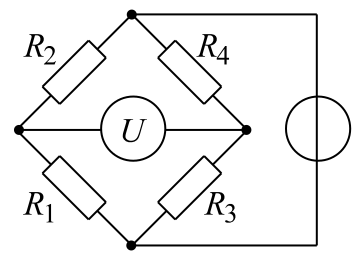
\includegraphics[width=0.4\textwidth]{../media/B1.5/WhBr_Diagonalbild.png}
	\caption{Schaltplan einer Wheatstonebrücke \cite{File:WhBr_Diagonalbild}}
\end{figure}

Durch das Oszilloskopsignal wird der Abgriff des Schleifdrahtes in die Mitte gebracht. Der Nullabgleich erfolgt dadurch, dass durch eine geeignete Wahl des Widerstandes $R_0$ und der Kapazität $C_0$ eines Kondensators das Signal am Oszilloskop auf ein Minimum gebracht wird. Der Feinabgleich erfolgt mit dem Schleifdraht.

Mithilfe der \emph{Wheatstoneformel} kann ein unbekannter Widerstand $R_x$ aus drei bekannten Widerständen $R_i$ bestimmt werden.

\begin{eqnarray}
    R_1 I_A &=& R_2 I_B \\
    R_3 I_A &=& R_4 I_B \\
    \Rightarrow \frac{R_1}{R_2} &=& \frac{R_3}{R_4}
\end{eqnarray}

\hypertarget{Versuchsaufbau}{\subsection{Versuchsaufbau}\label{Versuchsaufbau}}
Der in Abbildung \ref{fig:aufbau} dargestellte Versuchsaufbau besteht aus einem Resonator mit einer Brückenschaltung, welche mit hochfrequenter Wechselspannung von $146 \mathrm{\, MHz}$ betrieben wird.

Der eine Zweig dieser Brückenschaltung enthält einen variablen Widerstand, der andere einen abstimmbaren Schwingkreis. Der wiederum besteht aus einer Spule, in welcher sich die Probensubstanz befindet. Die Spule ist von zwei Helmholtzspulen umgeben umgeben.

Bei richtiger Einstellung ist die Impedanz beider Zweige gleich und es liegt keine Spannung am Diagonalzweig der Wheatstonebrücke an.

\begin{figure}[h!]
	\centering
	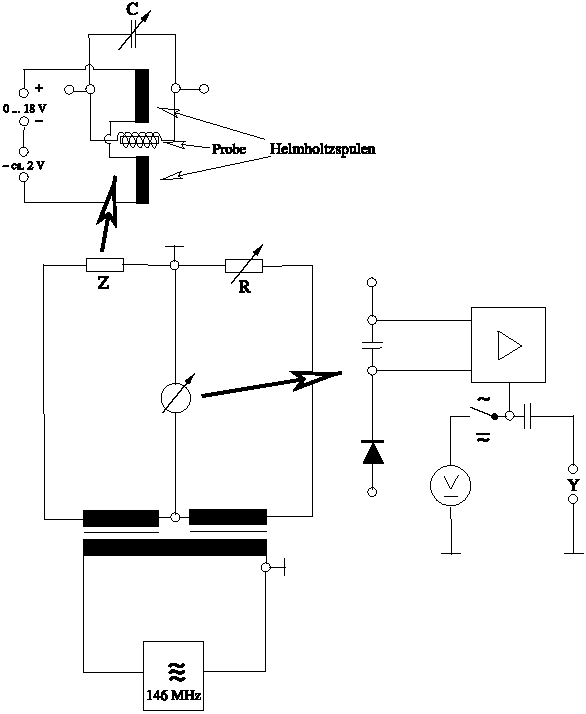
\includegraphics[width=0.7\textwidth]{../media/B1.5/Aufbau.pdf}
	\caption{Schaltplan der Brückenschaltung des Resonators \cite{Uni}}
	\label{fig:aufbau}
\end{figure}

Absorption von Strahlungsquanten beginnt dann in der Probe, wenn das Magnetfeld der Helmholtzspulen die Resonanzflussdichte $B_r$ erreicht. Damit ändert sich die Impedanz des Schwingkreises.

Am Diagonalzweig tritt eine Spannung auf, da beide Zweige der Brückenschaltung unterschiedliche Impedanzen haben. Diese Spannung wird mittels einer Halbleiterdiode gleichgerichtet und mit einem Kondensator verstärkt.

Falls die Gleichspannung an den Helmholtzspulen mit einer kleinen Wechselspannung überlagert wird, schwingt das dadurch erzeugte Magnetfeld. Bei geeigneter Einstellung oszilliert dieses symmetrisch um die Resonanzflussdichte $B_r$. Die mittels eines Multimeters gemessene mittlere Stromstärke entspricht dann genau der Resonanzstromstärke $I_r$.

\clearpage
\hypertarget{durchfuxfchrung}{\section{Durchführung}\label{durchfuxfchrung}}
Der Versuch besteht aus drei Teilen.

Im ersten Teil soll die Resonanzstromstärke $I_r$ ermittelt werden, um den Landé--Faktor eines Elektrons zu bestimmen, im zweiten die Halbwertsbreite des Signals. Diese beiden Versuchsteile werden gemeinsam ausgeführt, da sie die selbe Methodik verwenden. Weiterhin werden die Messungen jeweils fünf mal ausgeführt.

\subsection{Landé--Faktor}
\label{durchfuxfchrung:Lande-Faktor}
Ziel dieses Teils ist die Bestimmung des Landé--Faktor eines Elektrons in einer $\ce{DPPH}$--Probe.

Es wird ein Strom zwischen $1.0\mathrm{\, A}$ und $1.5 \mathrm{\, A}$ eingestellt. Die Kapazität des Resonators wird so konfiguriert, dass zwei möglichst symmetrische Glockenkurven auf dem Oszilloskop sichtbar sind. Dann wird die Phase so eingestellt, dass beide Kurven sich möglichst gut überlagern.

Mittels des Widerstandsreglers lässt sich die Amplitude der nun übereinander liegenden Glockenkurven maximieren. Daraufhin wird die Stromstärke so eingestellt, dass die Glockenkurven um die $y$--Achse zentriert sind. Diese eingestellte Stromstärke ist dann genau die gesuchte Resonanzstromstärke $I_r$. Daraufhin wird die Halbwertsbreite bestimmt, erst danach wird ein neuer Strom eingestellt.

\subsubsection{Halbwertsbreite}
\label{durchfuxfchrung:Halbwertsbreite}
Zur Bestimmung der Halbwertsbreite wird zunächst die halbe Höhe des Signals ermittelt, danach wird die dazugehörige Position bestimmt.

Dazu wird die Oszilloskopanzeige in $y$--Richtung verschoben, bis das Signal auf halber Höhe von der $x$--Achse geschnitten wird.  Daraufhin wird die sie in $x$--Richtung verschoben, bis das Signal den Ursprung schneidet. Das Signal wird erneut zentriert, indem die Stromstärke verändert wird.

Die Differenz der so gemessenen Stromstärke und der dazugehörigen Resonanzstromstärke $I_r$ entspricht der halben Halbwertsbreite.

\subsection{Erdmagnetfeld}
\label{durchfuxfchrung:Erdmagnetfeld}
Zur Messung des Erdmagnetfelds wird die Resonanzstromstärke $I_r$ für vier Ausrichtungen des Resonators gemessen. Dazu wird der Resonator in $90 \mathrm{\, ^\circ}$--Schritten rotiert. Für alle vier Richtungen werden jeweils fünf Messungen durchgeführt, wobei zwischen jeder Messung rotiert wird.

\clearpage
\hypertarget{auswertung}{\section{Auswertung}\label{auswertung}}

\subsection{Landé--Faktor}
\label{auswertung:Landé--Faktor}

Nun zur Bestimmung des g-Faktors von DPPH aus der gemessenen Resonanzstromstärke $I_r$. Dazu jedoch erst einige Überlegungen.

Durch die Kristallfelder in $\ce{DPPH}$ wird der Bahndrehimpuls des Elektrons fast völlig ausgelöscht, sodass ein reines Spinmoment $\vec{\mu}_s$ des Elektrons vorliegt. Dadurch kann die Energie $E$ des Elektrons im Magnetfeld bestimmt werden.

Sei die Richtung des konstanten Magnetfelds der Helmholtzspulen die $z$--Richtung. Dadurch wird die magnetische Flussdichte durch ihre $z$--Komponente bestimmt, wodurch nur die $z$--Komponente $\mu_{s,z}$ des magnetischen Moments die Energie des Elektrons beschreibt.

\begin{eqnarray}
	\vec{\mu}_\mathrm{ges} &=& \vec{\mu}_s \\
	E &=& \vec{\mu}_s \cdot \vec{B} \\
		&=& \mu_{s,z} \cdot B
\end{eqnarray}

\noindent
Durch die Definitionen des magnetischen Moments des Spins \eqref{eq:dipolmomentSpin} und durch das gyromagnetische Verhältnis \eqref{eq:gyromag} kann diese Relation umgeschrieben werden.

\begin{eqnarray}
	E &=& \gamma \cdot s_z \cdot B \\
		&=& \frac{g \cdot \mu_B}{\hbar} \cdot s_z \cdot B
\end{eqnarray}

\noindent
Weiterhin lässt sich $s_z$ durch die entsprechende magnetische Quantenzahl $m_s$ beschreiben, wie es in Abschnitt \ref{zeemanneffekt} beschrieben wurde. Hierbei ist $m_s$ durch die Forderung $|m_s|\le s$ eingeschränkt. Für Elektronen gilt daher $m_s=\pm\frac{1}{2}$.

\begin{eqnarray}
	s_z &=& \hbar \cdot m_s \\
	\Rightarrow E &=& g \cdot \mu_B \cdot m_s \cdot B
\end{eqnarray}

\noindent
Die Energiedifferenz $\Delta E$ zwischen den beiden Zuständen folgt aus der Differenz der magnetischen Spinquantenzahl $\Delta m_s = 1$.

Für die Anregung der Elektronen muss $\Delta E$ durch die Energie elektromagnetischer Strahlung \eqref{eq:Energie Strahlung} bereitgestellt werden.

\begin{eqnarray}
	\Delta E &=& g \cdot \mu_B \cdot B \label{eq:deltaE}
\end{eqnarray}

Dabei wird das entsprechende Resonanzmagnetfeld $B_r$ gemessen. Der Landé--Faktor $g$ folgt durch Gleichsetzen der Gleichungen \eqref{eq:deltaE} und \eqref{eq:Energie Strahlung}.

\begin{eqnarray}
	g &=& \frac{h \cdot \nu}{\mu_B \cdot B_r}
\end{eqnarray}

\noindent
Da das Magnetfeld der Helmholtzspulen ideal ist, wird ein Korrekturfaktor $\zeta$ verwendet. Dabei werden die Anzahl der Windungen $n_W$, der Spulenradius $r$, die magnetische Feldkonstante $\mu_0$ und die gemessene Resonanzstromstärke $I_r$ verwendet. Alle Konstanten sind in Tabelle \ref{table:konstanten} angegeben.

\begin{eqnarray}
	B_r &=& \zeta \cdot
			\left(\frac{4}{5}\right)^{\frac{3}{2}}
			\mu_0 \frac{n_W}{r} I_r
			\label{eq:b_r} \\
	\Rightarrow g &=& \frac{1}{\zeta} \cdot
			\left(\frac{5}{4}\right)^{\frac{3}{2}}
			\frac{h \nu r}{\mu_B \mu_0 n_W} \cdot \frac{1}{I_r}
			\label{eq:gFaktor}
\end{eqnarray}

\begin{table}[h!]
	\centering
	\begin{tabular}{c|c}
		Konstante & Wert \\
		\hline
		$\zeta$ & $0.90072$ \\
		$h$ & $6.6256 \cdot 10^{-34} \mathrm{\, Js}$ \\
		$\nu$ & $(146.000 \pm 0.012) \mathrm{\, MHz} $ \\
		$r$ & $0.054 \mathrm{\, m}$ \\
		$\mu_B$ & $9.2732 \cdot 10^{-24} \mathrm{\, Am^2}$ \\
		$\mu_0$ & $1.256 \cdot 10^{-6} \mathrm{\, Tm/A}$ \\
		$n_W$ & $250$ \\
	\end{tabular}
	\caption{Konstanten zur Bestimmung des Landé--Faktors nach Gleichung \eqref{eq:gFaktor}}
	\label{table:konstanten}
\end{table}

\noindent
$I_r$ wurde während des Versuchs fünf mal gemessen, um statistische Schwankungen zu minimieren. Die Ergebnisse sind in Tabelle \ref{table:I_r} dargestellt.

Daraus lässt sich der Mittelwert $\bar{I}_r$ inklusive Fehler $\Delta \bar{I}_r$ mittels folgender Formeln bilden.

\begin{eqnarray}
	\bar{I}_r &=& \frac{1}{5} \sum_{i=1}^{5} I_{r,i} \\
	\Delta \bar{I}_r &=& \pm\sqrt{\frac{1}{20} \sum_{i=1}^{5} (I_{r,i} - \bar{I}_r)^2} \\
	\Rightarrow \bar I_r &=& (1.24460 \pm 0.0012) \mathrm{\, A}
\end{eqnarray}

\begin{table}[h!]
	\centering
	\begin{tabular}{c|c}
		Messung & $I_r$ [A] \\
		\hline
		1 & $1.248$ \\
		2 & $1.243$ \\
		3 & $1.242$ \\
		4 & $1.243$ \\
		5 & $1.247$ \\
	\end{tabular}
	\caption{Messwerte der Resonanzstromstärke $I_r$}
	\label{table:I_r}
\end{table}

\noindent
Der Landé--Faktor $g\approx 2.2364$ folgt damit aus Gleichung \eqref{eq:gFaktor} inklusive eines Fehlers $\Delta g$ mittels Gauß'scher Fehlerfortpflanzung.

\begin{eqnarray}
	\Delta g &=&
		\pm\sqrt{
			\left(\frac{1}{\zeta} \left(\frac{5}{4}\right)^{\frac{3}{2}} \frac{h r \cdot \Delta \nu}{\mu_B \mu_0 n_W} \cdot  \frac{1}{I_r}\right)^2 + \left(\frac{1}{\zeta} \left(\frac{5}{4}\right)^{\frac{3}{2}} \frac{h \nu r}{\mu_B \mu_0 n_W} \cdot \frac{\Delta I_r}{I_r^2}\right)^2
		} \\
	g &=& 2.2364 \pm 0.0022
\end{eqnarray}

\noindent
Der Literaturwert für den Landé--Faktor in $\ce{DPPH}$ beträgt $2.0037$. \cite{Uni} Der hier bestimmte Wert stimmt auch innerhalb der Fehlergrenzen nicht damit überein.

Dies kann verschieden Erklärt werden. Zum Einen war die Einstellung des Signals am Oszilloskop recht ungenau. Das Signal zitterte stark und die beiden Signale ließen sich nicht perfekt in Phase bringen. Auch die die Symmetrie--Einstellung folgte nach Augenmaß.

Weitere Einflüsse sind durch das Erdmagnetfeld und die Halbwertsbreite des Signals. Diese werden in den folgenden Abschnitten genauer untersucht.

Insgesamt lässt sich sagen, dass das Messergebnis zumindest größenordnungsmäßig mit dem Literaturwert übereinstimmt und deshalb dieser Versuchsteil dennoch als Erfolg gewertet werden kann.

\subsection{Halbwertsbreite}
\label{auswertung:Halbwertsbreite}

Nun wird die Halbwertsbreite der Flussdichte $B_\mathrm{FWHM}$ aus der des Resonanzstroms $I_{r,\mathrm{FWHM}}$ ermittelt. Dafür wurden der Resonanzstrom $I_R$ und die Position der halben Halbwertsbreite $I_{r,\mathrm{FWHM}/2}$ gemessen, wie in Abschnitt \ref{durchfuxfchrung:Halbwertsbreite} beschrieben.

Der Fehler folgt aus Gauß'scher Fehlerfortpflanzung. Er kann vereinfacht werden, da der Fehler für alle Stromablesungen gleich ist. Die Messwerte sowie berechneten Halbwertsbreiten sind in Tabelle \ref{table:halbwertsbreiten} angegeben.

\begin{eqnarray}
	I_{r,\mathrm{FWHM}} &=& 2\cdot\left|I_r-I_{r,\mathrm{FWHM}/2}\right| \\
	\Delta I_{r,\mathrm{FWHM}} &=& \pm2\sqrt{2} \cdot \Delta I_r
\end{eqnarray}

\begin{table}[h!]
	\centering
	\begin{tabular}{c|c|c|c}
		Messung $i$ & $I_r$ $[\mathrm{A}]$ & $I_{r,\mathrm{FWHM}/2}$ $[\mathrm{A}]$ & $I_{r,\mathrm{FWHM}}$ $[\mathrm{mA]}$ \\
		\hline
		$1$ & $1.248 \pm 0.002$ & $1.222 \pm 0.002$ & $52 \pm 6$ \\
		$2$ & $1.243 \pm 0.002$ & $1.215 \pm 0.002$ & $56 \pm 6$ \\
		$3$ & $1.242 \pm 0.002$ & $1.270 \pm 0.002$ & $56 \pm 6$ \\
		$4$ & $1.243 \pm 0.002$ & $1.272 \pm 0.002$ & $58 \pm 6$ \\
		$5$ & $1.247 \pm 0.002$ & $1.217 \pm 0.002$ & $60 \pm 6$
	\end{tabular}
	\caption{Gemessene Resonanzstromstärken $I_r$, Positionen der\\
		halben Halbwertsbreite $I_{r,\mathrm{FWHM}/2}$ und Halbwertsbreiten $I_{r,\mathrm{FWHM}}$}
	\label{table:halbwertsbreiten}
\end{table}

Daraus wird der Mittelwert der Halbwertbreiten $\bar I_{r,\mathrm{FWHM}}$ bestimmt. Der Fehler $\Delta \bar I_{r,\mathrm{FWHM}}$ folgt aus der mittleren Quadratsumme der Residuen.

\begin{eqnarray}
	\bar I_{r,\mathrm{FWHM}} &=& \frac{1}{N} \sum_{i=1}^{N} I_{r,i,\mathrm{FWHM}}
	\label{eq:fwhmMittel} \\
	\Delta \bar I_{r,\mathrm{FWHM}} &=& \pm\sqrt{\frac{1}{N(N-1)}\sum_{i=1}^{N} (I_{r,i,\mathrm{FWHM}}-\bar I_{r,\mathrm{FWHM}})^2}
	\label{eq:fwhmMittelErr} \\
	\bar I_{r,\mathrm{FWHM}} &=& (56.40 \pm 1.76) \mathrm{\, mA}
\end{eqnarray}

\noindent
Die Halbwertsbreite der Flussdichte $B_\mathrm{FWHM}$ lässt sich somit inklusive Fehler $\Delta B_\mathrm{FWHM}$ nach Gauß'scher Fehlerfortpflanzung mittels Gleichung \eqref{eq:b_r} berechnen. Dabei wird $\bar I_{r,\mathrm{FWHM}}$ als Resonanzstrom verwendet. Die Konstanten sind wie in Abschnitt \ref{auswertung:Landé--Faktor} Tabelle \ref{table:konstanten} zu entnehmen.

\begin{eqnarray}
	B_{FWHM} &=& \xi \cdot \left(\frac{4}{5}\right)^{\frac{3}{2}}\mu _0 \frac{n_W}{r} \cdot \bar I_{r,\mathrm{FWHM}}
	\label{eq:b_fwhm} \\
	\Delta B_{FWHM} &=& \xi \cdot \left(\frac{4}{5}\right)^{\frac{3}{2}}\mu _0 \frac{n_W}{r} \cdot \Delta \bar I_{r,\mathrm{FWHM}} \\
	B_\mathrm{FWHM} &=& (2.11 \pm 0.07) \cdot 10^{-4} \mathrm{\, T}
\end{eqnarray}

\noindent
Der theoretische Wert beträgt $2.7 \cdot 10^{-4} \mathrm{\, T}$. \cite{Uni} Unser Ergebnis hat somit die selbe Größenordnung, stimmt mit dem theoretischen Wert aber auch innerhalb der Fehlergrenzen nicht überein.

Dies könnte ebenfalls am Schwanken des Resonanzsignals liegen. Es war aufgrund dieser Schwankung schwierig, die Stromstärke per Augenmaß genau einzustellen und zu justieren.

\subsection{Erdmagnetfeld}
Zuletzt wird der Betrag der horizontalen Komponente des Erdmagnetfeldes zum Magnetfeld bestimmt. Dieses überlagert sich mit dem Magnetfeld der Spule. Das gesamte Magnetfeld innerhalb der Spulen hängt von dem Winkel zwischen den Spulen und dem Erdmagnetfeld ab.

Die für alle vier Richtungen gemessenen Resonanzstromstärken $I_r$ sind in Tabelle \ref{table:erdmagnetfeldMessdaten} dargestellt. Als Orientierung ist die Position der Steuerungsknöpfe des Resonators angegeben. In den vorherigen Versuchsteilen waren diese nach vorne ausgerichtet, diese Position entspricht einer Rotation von $0\,^\circ$.

\begin{table}[h!]
	\centering
	\begin{tabular}{c|l|c}
		Messung $i$ & \multicolumn{1}{c|}{Orientierung} & Resonanzstrom $I_r$ $[\mathrm{A}]$ \\
		\hline
		1 & Knöpfe vorne & $1.246 \pm 0.002$ \\
		2 & Knöpfe rechts & $1.252 \pm 0.002$ \\
		3 & Knöpfe hinten & $1.243 \pm 0.002$ \\
		4 & Knöpfe links & $1.236 \pm 0.002$ \\
		5 & Knöpfe vorne & $1.245 \pm 0.002$ \\
		6 & Knöpfe links & $1.238 \pm 0.002$ \\
		7 & Knöpfe hinten & $1.244 \pm 0.002$ \\
		8 & Knöpfe rechts & $1.254 \pm 0.002$ \\
		9 & Knöpfe vorne & $1.247 \pm 0.002$ \\
		10 & Knöpfe links & $1.240 \pm 0.002$ \\
		11 & Knöpfe hinten & $1.245 \pm 0.002$ \\
		12 & Knöpfe rechts & $1.253 \pm 0.002$ \\
		13 & Knöpfe hinten & $1.244 \pm 0.002$ \\
		14 & Knöpfe links & $1.237 \pm 0.002$ \\
		15 & Knöpfe vorne & $1.247 \pm 0.002$ \\
		16 & Knöpfe rechts & $1.255 \pm 0.002$
	\end{tabular}
	\caption{Messung des Resonanzstrom bei verschiedenen Orientierungen;
		``Knöpfe~vorne"' entspricht $0\,^\circ$, alle Rotationen erfolgten um $90\,^\circ$}
	\label{table:erdmagnetfeldMessdaten}
\end{table}

Analog zu Abschnitt \ref{durchfuxfchrung:Halbwertsbreite} können die Resonanzstromstärken $\bar{I}_r$ und die entsprechenden magnetischen Flussdichten $B$ mittels der Gleichungen \eqref{eq:fwhmMittel}, \eqref{eq:fwhmMittelErr} und \eqref{eq:b_fwhm} ermittelt werden. Die Ergebnisse sind der Tabelle \ref{table:resonanzstromstärkeMittel} zu entnehmen.

\begin{table}[h!]
	\centering
	\begin{tabular}{l|c|c}
		Orientierung & $\bar{I}_{r}$ $[\mathrm{A}]$ & $B$ $[\mathrm{mT]}$ \\
		\hline
		Knöpfe vorne  & $1.2463 \pm 0.0005$ & $4.6705 \pm 0.0018$ \\
		Knöpfe rechts & $1.2535 \pm 0.0006$ & $4.6980 \pm 0.0024$ \\
		Knöpfe hinten & $1.2440 \pm 0.0004$ & $4.6620 \pm 0.0015$  \\
		Knöpfe links     & $1.2378 \pm 0.0009$ & $4.6390 \pm 0.0030$
	\end{tabular}
	\caption{mittlere Resonanzfrequenzen $\bar I_r$ und zugehörige Flussdichten $B$ bei verschiedenen Orientierungen;
		``Knöpfe~vorne"' entspricht $0\,^\circ$, alle Rotationen erfolgten um $90\,^\circ$}
	\label{tab:Erdmagnetfeld Ergebnisse}
\end{table}


Beim Betrachten der Werte fällt auf, dass $B_{vorne}$ und $B_{rechts}$ jeweils größer als $B_{hinten}$ und $B_{links}$ sind. Man kann sich die Felder wie in Abbildung \ref{fig:orientierungen} vorstellen, wobei die Länge der Pfeile hier nicht unbedingt mit dem Betrag der Vektoren übereinstimmt.

\begin{figure}[h!]
	\centering
	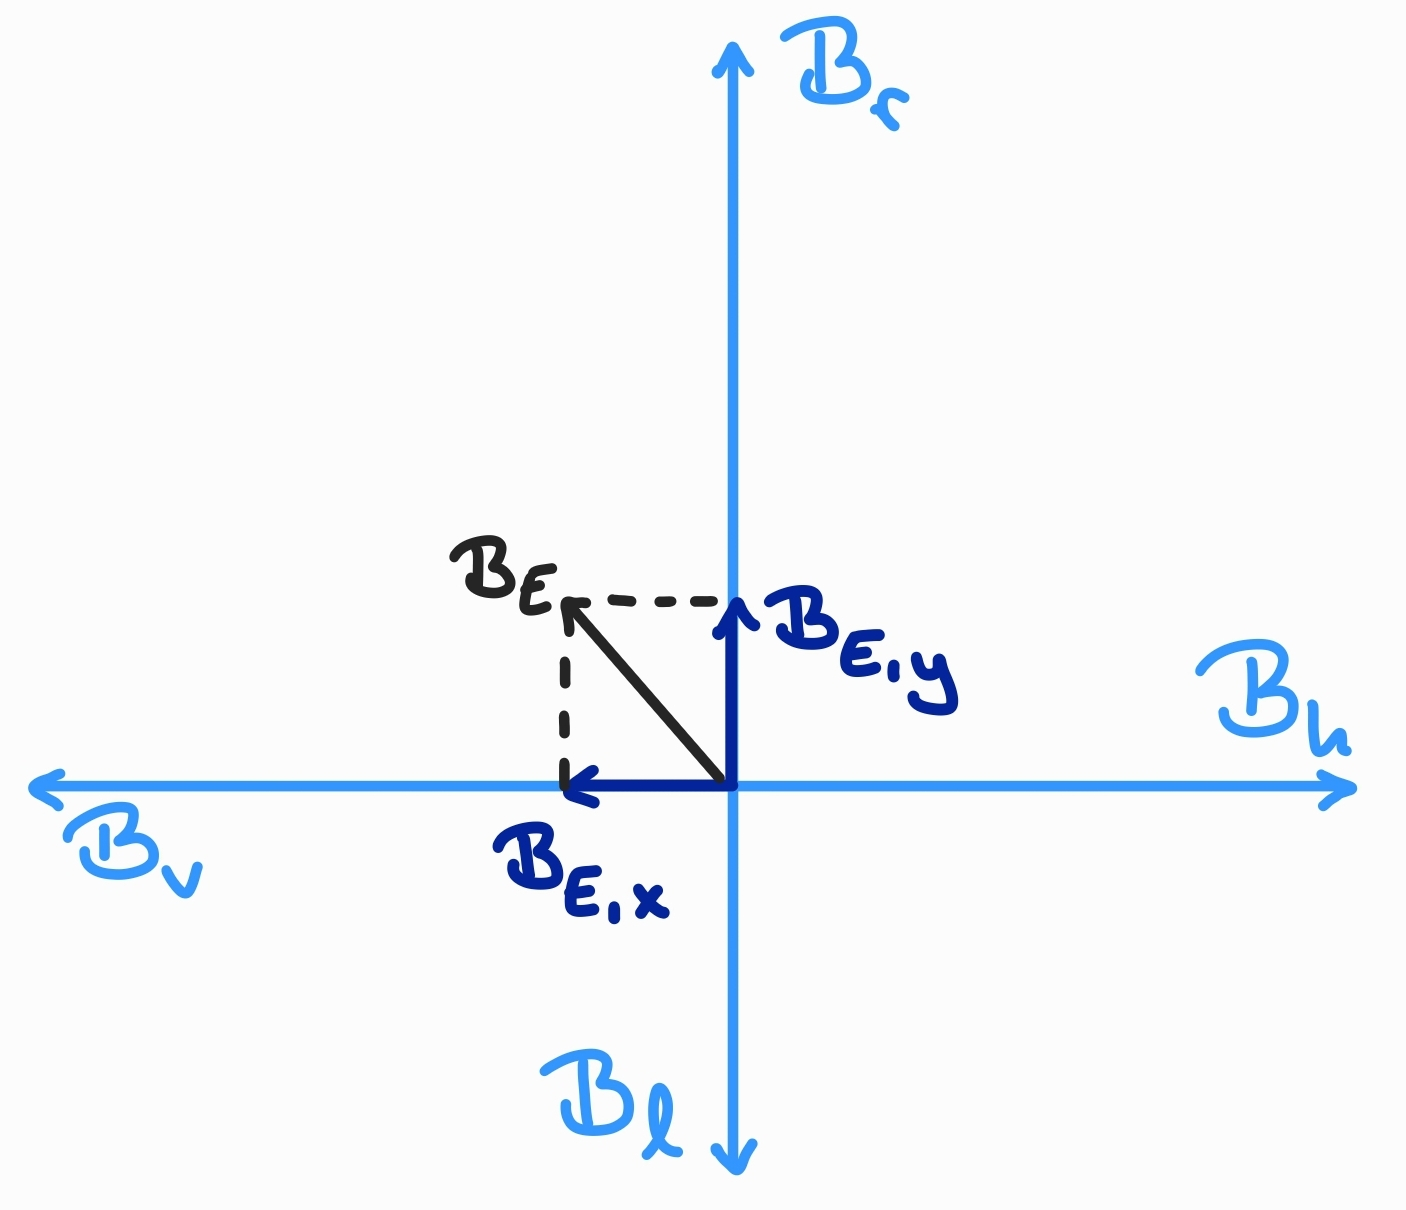
\includegraphics[scale=0.25]{../media/B1.5/Erdmagnetfeld.jpg}
	\caption{Visualisierung der verschiedenen Orientierungen}
	\label{fig:orientierungen}
\end{figure}

Die $x$-- und $y$--Komponenten des Erdmagnetfelds ergeben sich aus der halben Differenz der jeweiligen Komponenten der magnetischen Flussdichten zweier Orientierungen.

\begin{eqnarray}
	B_{\mathrm{Erde},x} &=& \frac{B_\mathrm{vorne}-B_\mathrm{hinten}}{2} \\
	B_{\mathrm{Erde},y} &=& \frac{B_\mathrm{rechts}-B_\mathrm{links}}{2} \\
	\Delta B_{\mathrm{Erde}, x} &=& \pm\sqrt{\left( \frac{\Delta B_\mathrm{vorne}}{2}\right) ^2 + \left( \frac{\Delta B_\mathrm{hinten}}{2}\right) ^2} \\
	\Delta B_{\mathrm{Erde}, y} &=& \pm\sqrt{\left( \frac{\Delta B_\mathrm{rechts}}{2}\right) ^2 + \left( \frac{\Delta B_\mathrm{links}}{2}\right) ^2} \\
	B_{\mathrm{Erde},x} &=& (4.21610 \pm 0.00117) \mathrm{\, mT} \\
	B_{\mathrm{Erde},y} &=& (29.51300 \pm 0.00192) \mathrm{\, mT}
\end{eqnarray}

\noindent
Das resultierende Erdmagnetfeld wird über den Satz des Pythagoras bestimmt.

\begin{eqnarray}
	B_\mathrm{Erde} &=& \sqrt{B_{\mathrm{Erde}, x}^2 + B_{\mathrm{Erde}, y}^2}\\
	\Delta B_\mathrm{Erde} &=& \pm\sqrt{\frac{(B_{\mathrm{Erde},x} \cdot \Delta B_{\mathrm{Erde}, x})^2 + (B_{\mathrm{Erde},y} \cdot \Delta B_{\mathrm{Erde}, y})^2}{B_{\mathrm{Erde}, x}^2 + B_{\mathrm{Erde},y}^2}}\\
	B_\mathrm{Erde} &=& (29.812 \pm 1.908) \cdot \mathrm{\, \mu T}
\end{eqnarray}

\noindent
Das gemessene Erdmagnetfeld beträgt somit $B_\mathrm{Erde} = (29.8 \pm 1.9) \mathrm{\,\mu T}$. In Köln beträgt die Stärke der horizontalen Komponente des Erdmagnetfeldes ungefähr $20 \mathrm{\,\mu T}$. \cite{Erdmagnetfeld}

Wie bei den vorherigen Versuchsteilen hier liegt der experimentelle Wert in derselben Größenordnung wie der Literaturwert, stimmt mit diesem aber auch innerhalb der Fehlergrenzen nicht überein.

Die Hauptfehlerquelle hier bleibt bei dem schwankenden Signal. Hinzu kommt, dass beim manuellen Drehen des Resonators per Hand der gewünschte Winkel von $90^{\circ} $ nicht exakt getroffen werden konnte. Da es keine Winkelskala gab, dürfte es einen merkbaren Fehler bei den Positionen geben. Dieser Faktor führt zu zusätzlichen Abweichungen in der Stromstärke.

\clearpage
\hypertarget{fazit}{\section{Fazit}\label{fazit}}
Insgesamt sind die Ergebnisse dieses Versuchs nur bedingt zufriedenstellend, da sie alle deutlich von den erwarteten Werten abweichen. Dafür stimmen sie zumindest größenordnungsmäßig mit den Theoriewerten überein. Somit ist der Versuch kein kompletter Fehlschlag.

Die zu identifizierende Abweichung des gemessenen Landé--Faktors vom Landé--Faktor vom theoretischen Wert ließ sich daher nicht nachweisen. Die Abweichung des gemessenen Landé--Faktors vom Literaturwert ist dafür zu groß. Dennoch stimmt der gemessene Landé--Faktor zumindest grob mit dem Literaturwert überein, wodurch dieser immerhin ungefähr nachgewiesen werden konnte.

Auch die Bestimmung der Halbwertsbreite lieferte eine recht große Abweichung vom erwarteten Wert, doch auch hier ließ sich der Wert wenigstens ungefähr nachweisen.

Zuletzt tritt auch bei der Bestimmung der magnetischen Flussdichte des Erdmagnetfeldes eine recht große Abweichung auf. Wieder stimmen aber Messwert und Literaturwert zumindest größenordnungsmäßig überein.

Für die Abweichungen aller drei Ergebnisse von den erwarteten Werten lassen sich mehrere Gründe finden. Zum Einen zitterte das Signal auf dem Oszilloskop während der Messung stark, weshalb eine genaue Einstellung desselben schwierig war. Des Weiteren ließen sich die beiden Glockenkurven nur mittelmäßig in Phase bringen.

Zudem folgte sämtliche Einstellungen der Signale nach Augenmaß, ebenso wie die Rotation des Resonators. Dadurch ist nur eine gewisse Präzision erreichbar. Rechnete man die Ungenauigkeit des Fehlers ein, so könnte das gemessene Erdmagnetfeld genauer mit dem Literaturwert übereinstimmen. Ebenso fließt die Beeinflussung des Erdmagnetfeldes nicht in die Bestimmung des Landé--Faktors ein. Unter dessen Berücksichtigung könnten möglicherweise bessere Ergebnisse bestimmt werden.

Trotz all den Abweichungen stimmen alle Messergebnisse größenordnungsmäßig mit den erwarteten Werten überein. Alle Ergebnisse lassen sich daher als bedingt erfolgreich bewerten, auch wenn die gewünschten Präzision nicht erreicht wurde.

\clearpage
\hypertarget{literatur}{%
\section{Literatur}\label{literatur}}
\renewcommand{\section}[2]{}

\begin{thebibliography}{99}
\bibitem{Jackson}
	J. D. Jackson, ``Classical Elektrodynamics'', 3. Auflage, Springer Verlag, 2018,
	DOI~\href{https://doi.org/10.1007/978-3-319-91809-9}{10.1007/978-3-319-91809-9}
	
\bibitem{Weber}
	R. Weber,  ``Atom-, Molekül- und Quantenphysik'', Teubner Verlag, 2007,
	ISBN: 978-3-8351-0201-9

\bibitem{Geomagnetismus}
	Physikalische--Technische Bundesanstalt, ``Geomagnetismus: Grundlagen zum Erdmagnetfeld'', \url{https://www.ptb.de/cms/fileadmin/internet/fachabteilungen/abteilung_2/2.5_halbleiterphysik_und_magnetismus/2.51/Geomagnetismus.pdf}, Abruf am 27.05.2024
	
\bibitem{Oldenburg}
	Universität Oldenburg, ``ESR--Stichworte'', 1995,
	\url{https://www.staff.uni-oldenburg.de/richard.kaupass/esr_stwo.html},
	Abruf am 27.05.2024
	
\bibitem{Bern}
	Universität Bern, ``ESR'', 1994, \url{https://www.physik.unibe.ch/e41821/e41822/e140946/e148625/e270487/files270492/Elektronenspinresonanz_ger.pdf},
	Abruf am 27.05.2024

\bibitem{Uni}
	Universität zu Köln, ``B1.5: Elektronenspinresonanz'', April 2024, Online verfügbar unter
	\url{https://teaching.astro.uni-koeln.de/sites/default/files/praktikum_b/Anleitung_1.5.pdf},
	Abruf am 17.04.2024

\bibitem{Radikale}
	Chemie.de, ``Radikale (Chemie)'',
	\url{https://www.chemie.de/lexikon/Radikale_(Chemie).html}, Abruf am 23.05.2024

\bibitem{Erdmagnetfeld}
	Deutsches GeoForschungsZentrum Potsdam, ``IGRF Declination Calculator'',
	\url{https://isdc.gfz-potsdam.de/igrf-declination-calculator/}, Abruf am 01.07.2024

\bibitem{File:WhBr_Diagonalbild}
	Wikimedia, ``File:WhBr\_Diagonalbild.svg'',
	\url{https://commons.wikimedia.org/wiki/File:WhBr_Diagonalbild.svg},
	Abruf am 23.05.2024

\end{thebibliography}
\end{document}
